
PWM (Pulse Width Modulation) é um modulação baseada na conversão linear de um valor em escala de tensão para outro em escala de \emph{Duty Cicle} aplicado a uma onda quadrada de amplitude qualquer. Este tipo de modulação é utilizada em diversas aplicações eletrônicas. 

\section{Modo de Funcionamento}

Para criar uma modulação PWM é necessário criar uma onda periódica linear e variante no tempo, que se consiga comparar com o sinal que se deseja converter em PWM. Logo o tipo de onda necessária neste modulação é a onda triangular ou a onda dente de serra. Para melhor compreensão a onda triangular ou dente de serra será denominada aqui de onda portadora, e o sinal ao qual se deseja converter em PWM será denominado sinal modulante.
  
Para a implementação digital deste método pode ser feito através uma comparação direta entre os módulos da onda portadora e o sinal modulante. Quando o modulo do sinal modulante for maior do que o  módulo da portadora  o sinal modulado vai para nível alto. Porém quando o módulo do sinal modulante for menor do que o módulo da portadora o sinal  modulado vai para zero. A grande diferença da implementação digital é que o sinal da portadora é gerado internamente através de um contador, que pode trabalhar no modo de contagem \emph{Down}, \emph{Up} ou \emph{UpDown}.

Quando o sinal da portadora é gerado através de um contador \emph{Down} ou \emph{Up}  a frequência do sinal modulado será igual a frequência do contador dividido pelo numero máximo de contagens. Já quando o sinal da portadora é gerador por um contador\emph{UpDown} a frequência do sinal modulado será igual a frequência do contador dividido por duas vezes o numero máximo de contagens. Sendo que o numero máximo de contagens deve ser maior ou igual ao modulo do sinal modulante. A Figura \ref{fig:Down} e a Figura \ref{fig:UpDown} apresentam melhor o modo como a geração de PWM é realizada digitalmente.  

\begin{figure}[H]
	\centering
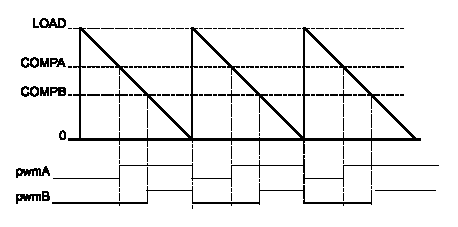
\includegraphics[width=0.8\textwidth] {figuras/Down.eps}
	\caption{PWM modo Down \cite{DATASHEET_TIVA}}
	\label{fig:Down}
\end{figure}

\begin{figure}[H]
	\centering
	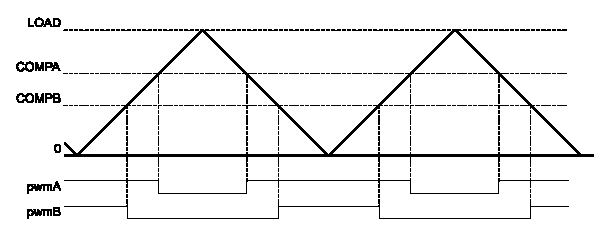
\includegraphics[width=0.8\textwidth] {figuras/UpDown.eps}
	\caption{PWM modo Down \cite{DATASHEET_TIVA}}
	\label{fig:UpDown}
\end{figure}

Tanto na Figura \ref{fig:Down} quanto na Figura \ref{fig:UpDown} os valores de \emph{LOAD}, \emph{COMPA}, \emph{COMPB}, \emph{pwmA} e \emph{pwmB} são referentes aos registradores presente do Tiva - TM4C1294NCPD, responsáveis pela modulação PWM. Tais registradores serão melhor abordados na próxima seção.  

\section{PWM do TM4C1294NCPDT}

O Tiva - TM4C1294NCPD possui um módulo PWM com quatro blocos geradores e seus respectivos blocos de controle, disponibilizando oito saídas PWM.  Através dos blocos de controle é possível escolher qual a polaridade de cada sinal PWM, e o seu respectivo pino. Cada bloco gerador produz 2 sinais PWM com a mesma frequência, porém ambos podem ter \emph{Duty Cicle} independentes ou \emph{Duty Cicle} complementares, com uma intervalo de \emph{Dead Band}. 

Como a maioria das aplicações com PWM é destinada ao chaveamento, o Tiva - TM4C1294NCPD possui não só uma configuração de geração PWM complementar com \emph{Dead Band}, recurso essencial para acionamento de pontes H, como também possui 4 pinos de entrada para um sistema de controle de falha, um para cada gerador PWM.

Para gerar a onda portadora o Tiva possui um contador de 16 bits capaz de realizar contagens no modo \emph{Down} e \emph{UpDown}, sendo possível atualizar o valor da contagem máxima (\emph{LOAD}). Cada um dos geradores PWM possuem ainda dois comparadores distintos (\emph{COMPA} e \emph{COMPB}), responsáveis por gerar os sinais PWM e que podem ser usados para gerar interrupções. 

Quando um comparador está configurado para provocar interrupções esta ocorre toda vez que o valor do comparador selecionado for maior do que o valor de \emph{LOAD}.  A Figura \ref{fig:PWMCountDownMode} demonstra o modo como as os sinais de interrupção são provocados pelos comparadores no modo \emph{Down}, e a Figura \ref{fig:PWMCountUpDownMode} demonstra o mesmo no modo \emph{UpDown}.

\begin{figure}[H]
	\centering
	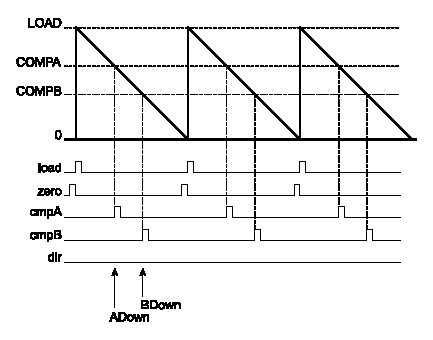
\includegraphics[width=0.8\textwidth] {figuras/PWMCountDownMode.eps}
	\caption{PWM modo Down \cite{DATASHEET_TIVA}}
	\label{fig:PWMCountDownMode}
\end{figure}

\begin{figure}[H]
	\centering
	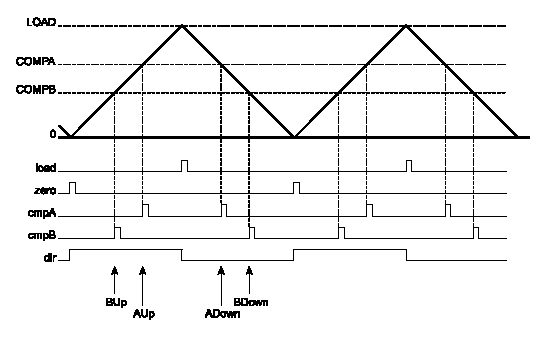
\includegraphics[width=0.8\textwidth] {figuras/PWMCountUpDownMode.eps}
	\caption{PWM modo Down \cite{DATASHEET_TIVA}}
	\label{fig:PWMCountUpDownMode}
\end{figure}

A tabela \ref{tab:CanaisPWM} apresenta os 8 pinos do módulo PWM, sendo estes pinos de saída dos sinais de PWM.  

\begin{center}
	\begin{longtable}{|c|c|c|c|c|}
		\rowcolor[HTML]{000000}
		{\color[HTML]{FFFFFF} Pino} & {\color[HTML]{FFFFFF} $n^{o}$} & {\color[HTML]{FFFFFF} Mux/Função} & {\color[HTML]{FFFFFF} Tipo} & {\color[HTML]{FFFFFF} Descrição}            \\
		M0PWM0    & 42  & PF0 (6) & O & Saída PWM 0\\
		M0PWM1    & 43  & PF1 (6) & O & Saída PWM 1\\
		M0PWM2    & 44  & PF2 (6) & O & Saída PWM 2\\
		M0PWM3    & 45  & PF3 (6) & O & Saída PWM 3\\
		M0PWM4    & 49  & PG0 (6) & O & Saída PWM 4\\
		M0PWM5    & 50  & PG1 (6) & O & Saída PWM 5\\
		M0PWM6    & 63  & PK4 (6) & O & Saída PWM 6\\
		M0PWM7    & 62  & PK5 (6) & O & Saída PWM 7\\
		\hline
		\caption{Canais PWM - Tiva TM4C1294NCPDT \cite{DATASHEET_TIVA} }
		\label{tab:CanaisPWM}
	\end{longtable}
\end{center}

\section{Na TivaWare}

As principais funções de configuração e utilização dos geradores de PWM e suas interrupções são listadas a seguir.

\begin{lstlisting}[style=funcao]
	void PWMClockSet(uint32_t ui32Base,
					 uint32_t ui32Config)
\end{lstlisting}

Configura a frequência do oscilador que alimenta a base de PWM especificada.

\begin{description}
	\item [\ttbu{ui32Base}]\hfill \\
	Base do gerador a ser configurado. Normalmente \textbf{PWM\emph{k}\_BASE}, onde \textbf{\emph{k}} é a letra identificadora do gerador.
	
	\item [\ttbu{ui32Config}]\hfill \\
	Divisão do clock do sistema, para a alimentação do gerador do PWM. É definida no formato \textbf{PWM\_SYSCLK\_DIV\_\emph{k}}, onde \textbf{\emph{k}} pode ser um dos valores: 1, 2, 4, 8, 16, 32 ou 64.
\end{description}

\begin{lstlisting}[style=funcao]
	void PWMGenConfigure(uint32_t ui32Base,
						 uint32_t ui32Gen,
						 uint32_t ui32Config)
\end{lstlisting}

Configura o gerador de PWM especificado.

\begin{description}
	\item [\ttbu{ui32Base}]\hfill \\
	Base do gerador a ser configurado. Normalmente \textbf{PWM\emph{k}\_BASE}, onde \textbf{\emph{k}} é o valor identificador do gerador.
	
	\item [\ttbu{ui32Gen}]\hfill \\
	Gerador a ser configurado. Definido por \textbf{PWM\_GEN\_\emph{k}}, onde \textbf{\emph{k}} pode ser um dos valores: 0, 1, 2 ou 3.
	
	\item [\ttbu{ui32Config}]\hfill \\
	Pacote de parâmetros em formato de OU lógico, onde cada parâmetro é representado no formato \textbf{PWM\_GEN\_MODE\_\emph{k}} e, k pode assumir os valores:
	\begin{itemize}
		\item \textbf{DOWN} ou \textbf{UP\_DOWN} para especificar o modo do contador.
		\item \textbf{SYNC} ou \textbf{NO\_SYNC} para especificar o modo de carregamento do contador e do comparador.
		\item \textbf{DBG\_RUN} ou \textbf{DBG\_STOP} para especificar o comportamento em tempo de depuração.
		\item \textbf{GEN\_NO\_SYNC}, \textbf{GEN\_SYNC\_LOCAL} ou \textbf{GEN\_SYNC\_GLOBAL} para especificar o modo de sincronização do contador do gerador.
		\item \textbf{DB\_NO\_SYNC}, \textbf{DB\_SYNC\_LOCAL} ou \textbf{DB\_SYNC\_GLOBAL} para especificar o modo de sincronização do parâmetro de \emph{deadband}.
		\item \textbf{FAULT\_LATCHED} ou \textbf{FAULT\_UNLATCHED} para especificar se falhas serão travadas ou não.
		\item \textbf{MINPER} ou \textbf{NO\_MINPER} para especificar se há ou não um período mínimo de falha.
		\item \textbf{FAULT\_EXT} ou \textbf{FAULT\_LEGACY} para especificar ou não o uso do suporte de seleção de fonte de falha estendida.
	\end{itemize}
	
\end{description}

\begin{lstlisting}[style=funcao]
	void PWMGenEnable(uint32_t ui32Base,
					   uint32_t ui32Gen)
\end{lstlisting}

Habilita o contador/gerador da base de PWM especificado.

\begin{description}
	\item [\ttbu{ui32Base}]\hfill \\
	Base do gerador a ser habilitado. Normalmente \textbf{PWM\emph{k}\_BASE}, onde \textbf{\emph{k}} é a letra identificadora do gerador.
	
	\item [\ttbu{ui32Gen}]\hfill \\
	Gerador a ser habilitado. Definido por \textbf{PWM\_GEN\_\emph{k}}, onde \textbf{\emph{k}} pode ser um dos valores: 0, 1, 2 ou 3.
\end{description}

\begin{lstlisting}[style=funcao]
	void PWMGenDisable(uint32_t ui32Base,
					   uint32_t ui32Gen)
\end{lstlisting}

Desabilita o contador/gerador da base de PWM especificado.

\begin{description}
	\item [\ttbu{ui32Base}]\hfill \\
	Base do gerador a ser desabilitado. Normalmente \textbf{PWM\emph{k}\_BASE}, onde \textbf{\emph{k}} é a letra identificadora do gerador.
	
	\item [\ttbu{ui32Gen}]\hfill \\
	Gerador a ser desabilitado. Definido por \textbf{PWM\_GEN\_\emph{k}}, onde \textbf{\emph{k}} pode ser um dos valores: 0, 1, 2 ou 3.
\end{description}

\begin{lstlisting}[style=funcao]
	void PWMGenIntTrigEnable(uint32_t ui32Base,
							 uint32_t ui32Gen,
							 uint32_t ui32IntTrig)
\end{lstlisting}

Configura os eventos que causam as interrupções no gerador da base de PWM especificada.

\begin{description}
	\item [\ttbu{ui32Base}]\hfill \\
	Base do gerador a ser configurado. Normalmente \textbf{PWM\emph{k}\_BASE}, onde \textbf{\emph{k}} é a letra identificadora do gerador.
	
	\item [\ttbu{ui32Gen}]\hfill \\
	Gerador a ser configurado. Definido por \textbf{PWM\_GEN\_\emph{k}}, onde \textbf{\emph{k}} pode ser um dos valores: 0, 1, 2 ou 3.
	
	\item [\ttbu{ui32Ints}]\hfill \\
	Pacote de parâmetros em formato de OU binário que especificam as interrupções do PWM. Cada parâmetro é representado no formato \textbf{PWM\_INT\_CNT\_\emph{k}}, onde \textbf{\emph{k}} pode assumir os valores:
	\begin{itemize}
		\item \textbf{ZERO} interrupção acionada ao zerar o contador.
		\item \textbf{LOAD} interrupção acionada ao chegar ao valor máximo do contador
		\item \textbf{AU} interrupção acionada quando o contador é incrementado e alcança o valor especificado no comparador A.
		\item \textbf{AD} interrupção acionada quando o contador é decrementado e alcança o valor especificado no comparador A.
		\item \textbf{BU} interrupção acionada quando o contador é incrementado e alcança o valor especificado no comparador B.
		\item \textbf{BD} interrupção acionada quando o contador é decrementado e alcança o valor especificado no comparador B.
	\end{itemize}
	
\end{description}

\begin{lstlisting}[style=funcao]
	void PWMGenIntClear(uint32_t ui32Base,
						uint32_t ui32Gen,
						uint32_t ui32Ints)
\end{lstlisting}

Limpa as \emph{flags} que marcam a ocorrência das interrupções especificadas no gerador da base de PWM especificado.

\begin{description}
	\item [\ttbu{ui32Base}]\hfill \\
	Base do gerador a ser configurado. Normalmente \textbf{PWM\emph{k}\_BASE}, onde \textbf{\emph{k}} é a letra identificadora do gerador.
	
	\item [\ttbu{ui32Gen}]\hfill \\
	Gerador a ser configurado. Definido por \textbf{PWM\_GEN\_\emph{k}}, onde \textbf{\emph{k}} pode ser um dos valores: 0, 1, 2 ou 3.
	
	\item [\ttbu{ui32Ints}]\hfill \\
	Pacote de parâmetros em formato de OU binário que especificam as interrupções do PWM. Cada parâmetro é representado no formato \textbf{PWM\_INT\_CNT\_\emph{k}}, onde \textbf{\emph{k}} pode assumir os valores:
	\begin{itemize}
		\item \textbf{ZERO} interrupção acionada ao zerar o contador.
		\item \textbf{LOAD} interrupção acionada ao chegar ao valor máximo do contador
		\item \textbf{AU} interrupção acionada quando o contador é incrementado e alcança o valor especificado no comparador A.
		\item \textbf{AD} interrupção acionada quando o contador é decrementado e alcança o valor especificado no comparador A.
		\item \textbf{BU} interrupção acionada quando o contador é incrementado e alcança o valor especificado no comparador B.
		\item \textbf{BD} interrupção acionada quando o contador é decrementado e alcança o valor especificado no comparador B.
	\end{itemize}
	
\end{description}

\begin{lstlisting}[style=funcao]
	void PWMGenIntRegister(uint32_t ui32Base,
						   uint32_t ui32Gen,
						   void (*pfnIntHandler)(void))
\end{lstlisting}

Configura a rotina de tratamento de interrupção do gerador da base de PWM especificada.

\begin{description}
	\item [\ttbu{ui32Base}]\hfill \\
	Base do gerador a ser configurado. Normalmente \textbf{PWM\emph{k}\_BASE}, onde \textbf{\emph{k}} é a letra identificadora do gerador.
	
	\item [\ttbu{ui32Gen}]\hfill \\
	Gerador a ser configurado. Definido por \textbf{PWM\_GEN\_\emph{k}}, onde \textbf{\emph{k}} pode ser um dos valores: 0, 1, 2 ou 3.
	
	\item [\ttbu{pfnIntHandler}]\hfill \\
	Ponteiro da função de tratamento. Esta não deve receber nada como parâmetro e nem retornar nada.
\end{description}

\begin{lstlisting}[style=funcao]
	void PWMGenPeriodSet(uint32_t ui32Base,
						 uint32_t ui32Gen,
						 uint32_t ui32Period)
\end{lstlisting}

Configura o período do sinal no gerador da base de PWM especificada.

\begin{description}
	\item [\ttbu{ui32Base}]\hfill \\
	Base do gerador a ser configurado. Normalmente \textbf{PWM\emph{k}\_BASE}, onde \textbf{\emph{k}} é a letra identificadora do gerador.
	
	\item [\ttbu{ui32Gen}]\hfill \\
	Gerador a ser configurado. Definido por \textbf{PWM\_GEN\_\emph{k}}, onde \textbf{\emph{k}} pode ser um dos valores: 0, 1, 2 ou 3.
	
	\item [\ttbu{ui32Period}]\hfill \\
	Período em formato de valor do contador entre 0 e 2$^n$- 1, onde \emph{n} é o número de bits do contador. Dado pela razão entre a frequência do clock do gerador e a frequência desejada para o PWM.
\end{description}

\begin{lstlisting}[style=funcao]
	void PWMIntEnable(uint32_t ui32Base,
					  uint32_t ui32GenFault)
\end{lstlisting}

Habilita as interrupções para o gerador da base de PWM especificada.

\begin{description}
	\item [\ttbu{ui32Base}]\hfill \\
	Base do gerador a ser configurado. Normalmente \textbf{PWM\emph{k}\_BASE}, onde \textbf{\emph{k}} é a letra identificadora do gerador.
	
	\item [\ttbu{ui32GenFaults}]\hfill \\
	Pacote de parâmetros em formato de OU binário que especificam os geradores que causam interrupções do PWM. Cada parâmetro é representado no formato \textbf{PWM\_INT\_GEN\_\emph{k}}, onde \textbf{\emph{k}} pode assumir os valores: 0, 1, 2, 3.
\end{description}

\begin{lstlisting}[style=funcao]
	void PWMIntDisable(uint32_t ui32Base,
					  uint32_t ui32GenFault)
\end{lstlisting}

Desabilita as interrupções para o gerador da base de PWM especificada.

\begin{description}
	\item [\ttbu{ui32Base}]\hfill \\
	Base do gerador a ser configurado. Normalmente \textbf{PWM\emph{k}\_BASE}, onde \textbf{\emph{k}} é a letra identificadora do gerador.
	
	\item [\ttbu{ui32GenFaults}]\hfill \\
	Pacote de parâmetros em formato de OU binário que especificam os geradores que causam interrupções do PWM. Cada parâmetro é representado no formato \textbf{PWM\_INT\_GEN\_\emph{k}}, onde \textbf{\emph{k}} pode assumir os valores: 0, 1, 2, 3.
\end{description}

\begin{lstlisting}[style=funcao]
	void PWMPulseWidthSet(uint32_t ui32Base,
						  uint32_t ui32PWMOut,
						  uint32_t ui32Width)
\end{lstlisting}

Desabilita as interrupções para o gerador da base de PWM especificada.

\begin{description}
	\item [\ttbu{ui32Base}]\hfill \\
	Base do gerador a ser configurado. Normalmente \textbf{PWM\emph{k}\_BASE}, onde \textbf{\emph{k}} é a letra identificadora do gerador.
	
	\item [\ttbu{ui32PWMOut}]\hfill \\
	Valor que representa a saída de PWM a ser configurada. Representado no formato \textbf{PWM\_OUT\_\emph{k}}, onde \textbf{\emph{k}} pode assumir valores de 0 à 7.
	
	\item [\ttbu{ui32Width}]\hfill \\
	Valor do contador em que o sinal ficará em nível alto.
\end{description}

\section{Exemplo}

Um exemplo de configuração de PWM, utilizando a saída 0 do gerador 0 é apresentada a seguir. É gerada uma onda quadrada de 10 KHz. Outro exemplo, utilizando a interrupção do PWM, pode ser
 encontrado na Seção \ref{sec:exPwm}.
 
\begin{lstlisting}[style=citacao]
	// Configura clock do sistema de 120 MHz
	SysCtlClockFreqSet((SYSCTL_XTAL_25MHZ | SYSCTL_OSC_MAIN | 
		SYSCTL_USE_PLL | SYSCTL_CFG_VCO_480), 120000000);
	// Habilita o PWM 0
	SysCtlPeripheralEnable(SYSCTL_PERIPH_PWM0);
	// Habilita a porta F utilizada no pino de saida de PWM
	SysCtlPeripheralEnable(SYSCTL_PERIPH_GPIOF);

	// Habilita pino de saida1 do PWM 0
	GPIOPinConfigure(GPIO_PF1_M0PWM1);
	// Configura pino F1 como saida do PWM
	GPIOPinTypePWM(GPIO_PORTF_BASE, GPIO_PIN_1);

	// PWM no gerador 0 em modo regressivo, nao sincronizado
	PWMGenConfigure(
		PWM0_BASE, PWM_GEN_0, PWM_GEN_MODE_DOWN |
		PWM_GEN_MODE_NO_SYNC);
	// CLock do gerador e o do sistema dividido por 4
	PWMClockSet(PWM0_BASE, PWM_SYSCLK_DIV_4);
	// Periodo de 10 KHz -> 120000000 / 4 / 10000
	PWMGenPeriodSet(PWM0_BASE, PWM_GEN_0, 3000);
	// Largura de pulso de 50% -> 3000 * 0.5
	PWMPulseWidthSet(PWM0_BASE, PWM_OUT_1, 1500);
	// Habilita gerador 0
	PWMGenEnable(PWM0_BASE, PWM_GEN_0);
	// Saidas de PWM a serem modificadas
	PWMOutputState(PWM0_BASE,
		(PWM_OUT_0_BIT | PWM_OUT_1_BIT), true);
	
	// Habilita interrupcao do gerador 0
	PWMIntEnable(PWM0_BASE, PWM_INT_GEN_0);
	// Habilita interrupcao do PWM 0
	IntEnable(INT_PWM0_0);
	// Interrupcao disparada no estouro do contador
	PWMGenIntTrigEnable(PWM0_BASE, PWM_GEN_0, 
		PWM_INT_CNT_LOAD);
\end{lstlisting}